\documentclass[letterpaper,12pt,smallheadings]{scrartcl}
\usepackage[margin=1in]{geometry}

%\usepackage{pdftex}
%\usepackage[pdftex]{graphicx}
\usepackage{graphicx}
\usepackage{jurabib}

\usepackage{setspace}
\doublespace



%\usepackage[small,compact]{titlesec}

%%% headings
\usepackage{fancyhdr}
\pagestyle{fancy}
\lhead{SCCC 05-11A}
\chead{}
\rhead{\thepage}
\lfoot{}
\cfoot{}
\rfoot{}
\renewcommand{\headrulewidth}{0.4pt}
%%%

% For Times (Nimbus Roman) Font:
\usepackage[T1]{fontenc}
\usepackage{mathptmx}

%\jurabibsetup{
%	citefull=first,
%	ibidem=strict,
%	commabeforerest,
%}
\jurabibsetup{
        %authorformat=smallcaps,
        authorformat={year,and},%authorformat=and,      authorformat=year,
        round,
        titleformat=italic,%
        titleformat=all,%
        titleformat=commasep,%
        commabeforerest,%
        ibidem=strict,%
        bibformat=ibidem,% bibformat=compress,%
        bibformat=raggedright,
        dotafter=bibentry,
        %pages=format,%
}

\renewcommand{\bibansep}{, }                    % Want a comma instead of a colon after the Author:
%\jbyearaftertitle
%\renewcommand{\jbcitationyearformat}[1]{#1}
%\renewcommand{\bibansep}{, }
%\renewcommand{\bibatsep}{.}
%\renewcommand{\bibapifont}{\textit}
%\renewcommand{\biblnfont}{}
%\renewcommand{\bibfnfont}{}
%\renewcommand{\bibelnfont}{}
%\renewcommand{\bibefnfont}{}
%\renewcommand{\bibtfont}{\textit}
%\renewcommand{\bibbtfont}{\textit}
%\renewcommand{\bibjtfont}{}

\newenvironment{blkquote}[1][1]
    { \begin{quote}\begin{spacing}{ #1}\small }
        { \end{spacing}\end{quote} \vspace{-24pt} }
\deffootnote{1.5em}{1em}{%
        \makebox[1.5em][l]{\thefootnotemark}}




\begin{document}
\pagenumbering{roman}
\singlespace
\thispagestyle{empty}
\begin{titlepage}
	\begin{center}
		BATTLE ANALYSIS\\
		\vspace{3em}
		THE BATTLE OF COWPENS\\
		\vspace{3em}
		SCCC CLASS \#05-11, GROUP \#1\\
		\vspace{3em}
		Alvarado\\
		\vspace{1em}
		Allen\\
		Bieber\\
		C.\\
		Flores\\
		Futch\\
		Hudak\\
		Kalmus\\
		Nagle\\
		Nicholson\\
	\end{center}
\end{titlepage}

\tableofcontents
\newpage
\pagenumbering{arabic}

\section{Introduction}


This is a change via git hub. Delete me later.

\subsection{Annotated Bibliography}

\nocite{*}
\bibliographystyle{jurabib}
%\bibliographystyle{annotate}
\bibliography{99-references}

\section{The Strategic Setting}

\subsection{Causes of the Conflict}

Causes\ldots

\subsection{Comparison of the Antagonists}

Overview text goes here.

\begin{table}
\caption{Main aspects of the antagonists.}
\begin{tabular}{p{2in}p{2in}p{2in}}
Factor				&	Colonies	& British	\\\hline
National (Strategic) objectives	&			&		\\
Insturments of National Power	&			&		\\
Military Systems		&			&		\\
Previous performance		& French and Indian War	&		\\
\end{tabular}
\end{table}

\subsubsection{National (Strategic) objectives}

Some text.

\subsubsection{Insturments of National Power}

Some text.

\subsubsection{Military Systems}

Some text.

\subsubsection{Previous performance}

Some text.


\section{The Operational Situation}

Overview

\subsection{The Context Within the Campaign}

\subsection{Operational Themes (FM 3-0)}

\subsection{Campaign Objectives}

\subsection{Operational Events Leading to the Battle}

Chronology here.

\begin{figure}[h!]
\centering
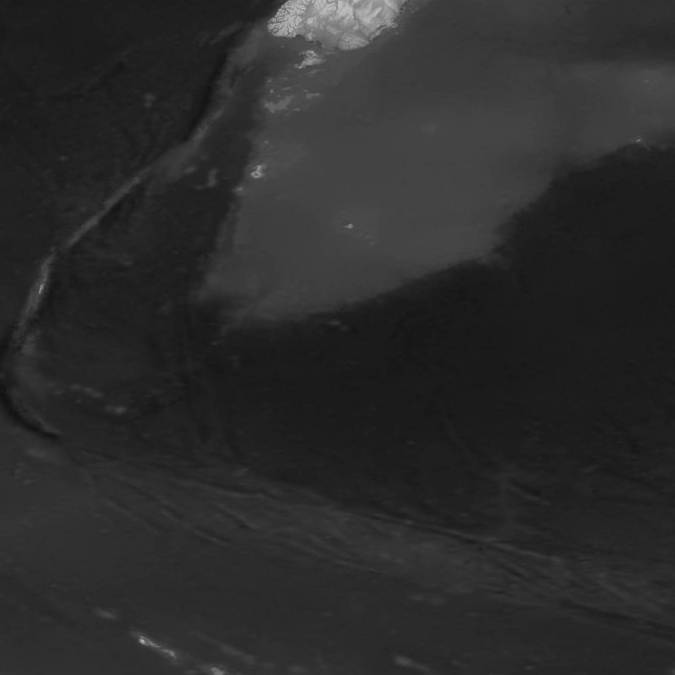
\includegraphics[width=0.8\textwidth]{gfx/map1}
\caption{map of \ldots}
\end{figure}




\section{The Tactical Situation}


\subsection{The Area of Operations}

%\subsubsection{Climate and Weather}

Due to the nature of the battle reports and personal anecdotes of the
participants, there is not a great deal of information regarding the climatology
and weather conditions of the Battle of Cowpens.  However, a historical analysis
by the South Carolina State Climatology Office indicates a January average
minimum temperature of 25$^\circ$ Fahrenheit and average maximum of 50$^\circ$ Fahrenheit from
1971 to 2000 for the area surrounding the battle (SCSCO).  For the purposes of
this paper it will be assumed that this trend also applies for the month of
January 1781.

\begin{quote}
``It was a bitter cold morning, and the soldiers slapped their hands to keep warm
as they waited in the dark for the British troops to arrive.  No evidence
remains of the time the engagement began; not even the sun would signal the
onslaught on this overcast day'' \cite[51]{moncure_cowpens_1996}.  This statement, along with
others, indicate that it was a very cold, overcast day; this low  temperature
and high humidity would have affected the combatants by stiffening their fingers
and joints, slowing marching speeds, and hindering fine muscle movements, such
as reloading their weapons and fixing bayonets. Soldiers were not alone in being
impacted by the cold and damp, their equipment also suffered.  ``Dampness made it
difficult for flintlocks to fire or to ignite rapidly, affecting accuracy'' \cite[79]{babits_devil_2001}.
It would also have had a negative outcome upon morale. 
Visibility on both sides was limited: ``Low clouds or mist affected any
assessment of troop dispositions, even after full daylight.  Combined with
ground cover and elevation, mist may have blocked Tarleton's ability to see the
Continentals waiting on the main line'' \cite[80]{babits_devil_2001}.
\end{quote}

The climate on the morning of the battle appears to have benefited the
Continentals in that, even though both forces had to face the hardships of
weather, the Americans had been able to rest, unlike Tarleton's forces who had
to march all night to meet them at Cowpens.  Tarleton’s men were likely feeling
the greater effects of the cold.  It also mitigated another concern for Morgan:
his men would have been looking directly into the sun during the battle, had the
day not been overcast: “Clouds benefited the Americans, who would otherwise have
had the early morning sun in their eyes.” \cite[67]{moncure_cowpens_1996}.  

\subsubsection{Terrain}

The landscape at Cowpens, given current advances in tactics and technology,
would be considered a ``killing ground'' or optimal ambush point.  Considering the
equipment and combat tactics of the time, it was a perfectly suited battleground
for the forces involved.  Tarleton considered it ``An open meadow (for cattle
grazing) about 500 yards deep and the same wide, gently undulating, not much in
the way of trees and undergrowth; good terrain to maneuver infantry; good space
to use cavalry once the enemy was broken.  The Mill Gap road bisected the field
North to South'' \cite[326]{stephenson_patriot_2007}.
From Morgan's perspective the landscape was ``relatively flat open ground
sparsely scattered with red oak and pine, the site was ideal for grazing cows or
fighting European style battles.  From the direction the British must come
(Northwest along Mill Gap Road), a single trail opened into a narrow plain that
sloped gently but unevenly uphill to the center of the pens'' \cite[45]{moncure_cowpens_1996}.
The only avenue of approach for the British was the Mill Gap Road, a trail that
had become extremely muddy due to recent rains in the region. ``The advance of
the British in the dark across a country cut by ravines and swollen, muddy
creeks was slow'' \cite[126]{lumpkin_savannah_1981}.  Figure \ref{terrain1a}
shows the terrain surrounding the battle site.  

\begin{figure}[ht]
    \begin{center}
    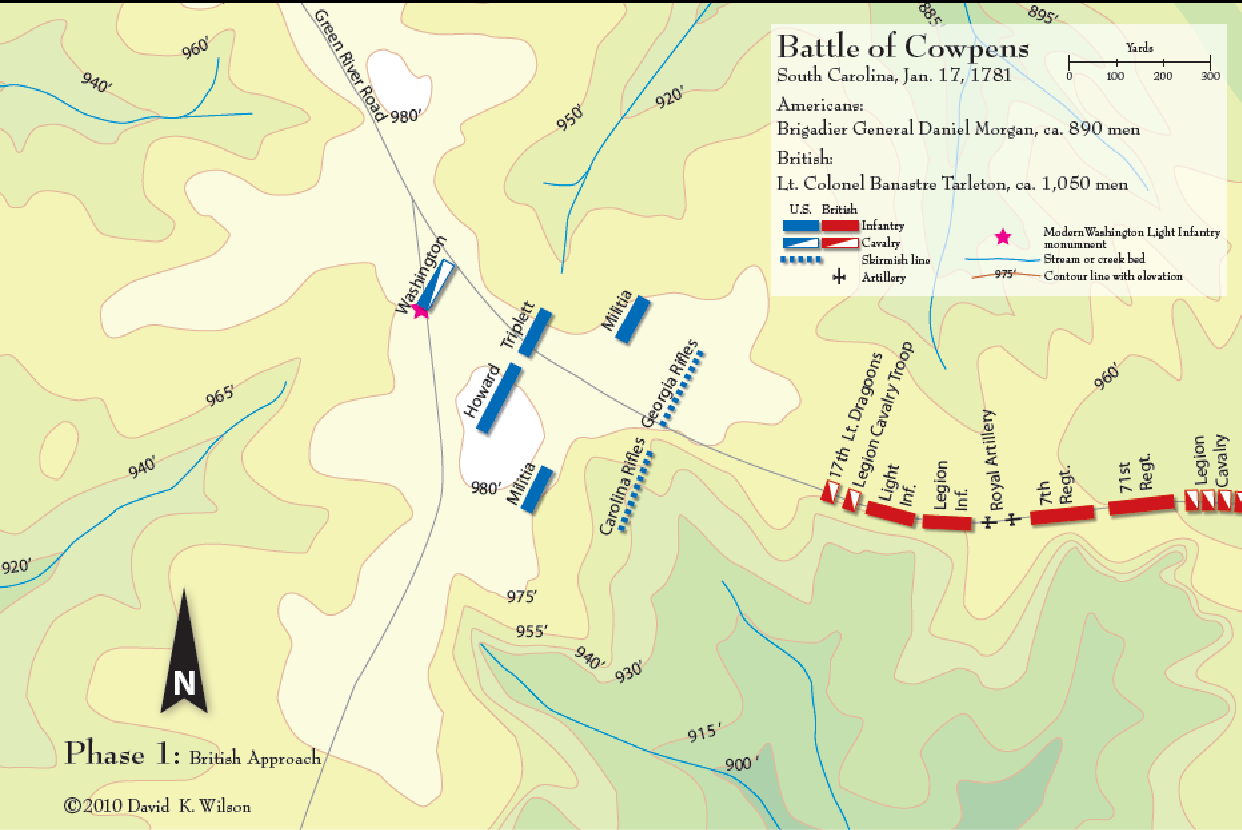
\includegraphics[width=\textwidth]{gfx/futch1}
    \end{center}
    %\caption{Terrain overview of the Battle of Cowpens. \cite{wilson_blogmap}}
    \caption{Phase 1: British approach at Cowpens. \cite{wilson_blogmap}}
	%\url{http://www.davidwilsonhome.com/homepage/Perspectives/Entries/2010/4/11_The_Battle_of_Cowpens__A_Cartographic_Interpretation.html)}
    \label{terrain1a}
\end{figure}

Morgan, in seizing what limited high ground there was, had the advantage of
Tarleton in regards to observation during the British infiltration, but any
benefit was negated during the battle due to the gently sloping terrain once
Tarleton’s forces had entered the meadow.  The British’s cannons were not
influenced by the terrain at all. 

For a relatively small battlefield, there was a great deal of important or key
terrain to be had.  One of the primary ones was a series of crests near the
center of the field: “They found a slope lightly forested in hardwoods and pine,
possibly 150 yards long. This rose to a low ridge, dipped down to a shallow
swale, and rose again to a higher ridge.  Just behind the crown of the second
ridge was a deeper gully in which cavalry might be concealed.  The depth of the
second draw was such that horsemen could rise in their stirrups and see all the
way down the slope to the forest from which the British must come”
\cite[126]{lumpkin_savannah_1981} \cite[126]{lumpkin_savannah_1981}.
This saddle in between two crests was the perfect depth to both shield
cavalry from attacking forces and to allow them visibility of the battle with
little effort. Another piece of key terrain was the marshland that braced both
sides (east and west) of the Continental line.  ``The flanks were close to the
marshy ground of two creeks that bracketed the Cowpens'' \cite[327]{stephenson_patriot_2007}.
The marsh on both sides of the battlefield created a canalization effect for the
attacking British, limiting their ability to flank the Continental forces.  

Operationally, the terrain had a different impact for each side.  Morgan used
the gully to obscure his cavalry and the marshes on either side of his forces to
limit the possibility of an enemy flank.  Tarleton appears to have disregarded
those factors and did not account for their impact during the battle.  “Morgan
noted the way the land fell off to the left and right toward several creeks.
The Cowpens was bordered by marshy ground that would make it difficult for
Tarleton to execute any sweeping flank movements with his cavalry” \cite[45]{fleming_cowpens_1988}.

The aforementioned marshes were a key obstacle in the fight, hemming and
canalizing the British into fighting straight on and limiting any flanking
movements.  That being said, the area in which the majority of the fighting took
place in was ``an open rolling woodland of first-growth pines and hardwoods,
excellent country for cavalrymen but with very little cover for riflemen''
\cite[124]{lumpkin_savannah_1981}.  The terrain definitely influenced the battle, it allowed
Morgan to anchor his forces to the low hill in the center and tie them into the
edge of a marsh on the eastern side of the battleground, and it led Tarleton to
make an assumption that this fight was going to be fought the way he was
accustomed to: ``the ground was optimal for Tarleton's cavalry, as the British
commander noted, although it sloped gently upward toward the American forces''
\cite[46]{moncure_cowpens_1996}.

Given the nature of the terrain and the style of warfare at the time, there was
not much in the way of cover or concealment to be had.  In fact, ``all sources
agree the battlefield was partially open with `not one single bush on the field
of battle to entangle the troops.'''\cite[66]{babits_devil_2001}.  Morgan made
excellent use of the dip in elevation behind his troops: ``Behind the main line,
in a shallow gully, Morgan parked William Washington's 3rd Continental Light
Dragoons (82 men) together with 45 volunteer horsemen drawn from the militia''
\cite[327]{stephenson_patriot_2007}.  The lack of cover or concealment clearly
led Tarleton to believe that this fight would be on his terms and fought in a
manner in which he was familiar.  


%\paragraph{Observation and Fields of Fire}
%
%\ldots
%
%\paragraph{Avenues of Approach}
%
%\ldots
%
%\paragraph{Key Terrain}
%
%\ldots
%
%\paragraph{Obstacles}
%
%\ldots
%
%\paragraph{Cover and Concealment}
%
%\ldots
%
%\subsection{Comparison of Opposing Forces}
%
%\ldots

\subsubsection{Strength and Composition}


At the Battle of Cowpens, the British had approximately 1000 - 1200 troops.
Tarleton’s force consisted of “550 dragoons and light infantry of the British
Legion, the 1st Battalion of the 71st Foot (200 men), a similar number of the
7th Foot, 50 horsemen of the 17th Dragoons, and a 50-man contingent of the Royal
Artillery with two three-pound grasshoppers; in all, just over 1,000 men”
\cite[p.325]{stephenson_patriot_2007}.  The 7th Foot was commanded by Major Timothy Newmarsh.  It
was comprised of about 168 men arranged in four companies.  The 71st Foot was
known as Fraser’s Highlanders and was raised specifically for American service
in 1775.  At the Battle of Cowpens the 71st Foot was comprised of 249 men and 14
officers.  British companies had approximately forty men in each company.  The
British Legion Infantry was comprised of 200 – 271 enlisted Infantry men and
nearly 250 horsemen. It was normally commanded by MAJ George Hanger however he
was absent due to sickness at the time of Cowpens, his most likely replacement
was Captain John Rousselet.  The 17th light Dragoons consisted of 50 horsemen
commanded by Lieutenant Henry Nettles.        

The   Continental Army outnumbered the British army by just a little bit.  It is
estimated they had between 1,100 – 1,300 troops under the command of Morgan.
Even though the Continental Army outnumbered the British, they were not as well
equipped, trained, or experienced giving the British the advantage as to troops.
The most experience troops Morgan had were the 300 man Battalion of Continental
troops received from General Greene.  The battalion of consisted of 5 companies
and each company was comprised of 60 men.  The battalion of continental troops
was commanded by LTC John Eager Howard of Baltimore.  Daniel Morgan received the
cream of the crop of these troops.  The rest of his army consisted of 82 light
dragoon riders that were greatly under equipped and under strength along with
militia forces that came scattered throughout the area.  “In addition to
Continental light infantry, a Virginia militia battalion under Major Francis
Triplett saw extensive service with the flying army.  North Carolina militiamen
under Colonel Joseph McDowell operated a second militia battalion under Morgan.
Finally, cavalry composed largely of the remnants of the Third Continental
Dragoons under William Washington completed the components of the Flying Army”
\cite[p.25]{babits_devil_2001}.

\subsubsection{Weapsons Technology}


The types of weapons both the British and Continental Armies used in the
revolutionary war played critically as to how battles were fought and won.  Each
Army had different advantages over the other in types of weapons they used.  The
British had standard weapons throughout its troops while the Continental had a
vast variety of weapons. The weapons comprised at the Battle of Cowpens
included, muskets, rifles, sabers, carbines, bayonets and artillery cannons.  

The Continental Infantrymen mainly carried a French Smoothbore musket with a
bayonet attached.  These French muskets were loaded with a .69 caliber round
with was .63 inches in diameter.  A smoothbore musket has no rifling and does
not allow the projectile to spin extremely diminishing the accuracy of the
round.  In 1777, General George Washington ordered the use of buckshot to be
used, meaning buckshot was used at the Battle of Cowpens.  “Buckshot consisted
of one large ball and at least three small (.30 Caliber) balls.  This allowed
one single Company of 60 men to launch 240 projectiles in 1 single volley”
\cite[p.12]{babits_devil_2001}.  The technique greatly enhanced the amount of firepower of one
company allowing four times as much damage per volley.

The British Infantrymen also carried muskets referred to as the Brown Bess.
These weapons were British made and used a .75 caliber round and had a 17 inch 3
sided bayonet attached.  The three sided bayonet would cause more damage than a
bladed bayonet by creating a larger hole in their opponents’ body.  This made it
much harder for anyone to close the wound allowing it to heal.  The British
Officers and Non Commissioned Officers carried swords with them.  Many British
Officers would also carry spontoons.

The Continental Cavalrymen were not equipped as well as the British Cavalrymen.
The primary weapon of the Cavalrymen was their sabers.  “The militia obtained
sabers by going to all the sawmills.  They would take all the old whip saws and
set three of four smiths to work to create a Saber.  Most swords were polished
with Grindstone” \cite[p.21]{babits_devil_2001}.  This reference shows that the Continental Army
had to be very resourceful when it came to sabers.  Cavalrymen would also carry
a .67 caliber French Carbine.  The handguns were nine inches in barrel length.
It is estimated that for every four Continental Cavalrymen only one would have a
carbine.

The British Cavalry, also referred to as dragoons, were much better equipped
than the Continentals.  Each rider carried a saber that was long, heavy and had
a deeply curved blade like a crescent.  Each Saber had a single edge and a
knuckle guard to protect the rider’s hand.  Each British Cavalrymen also carried
a short musket or a carbine.  These carbines carried a .62 or .65 caliber round.
Even though each rider had a carbine, these weapons were not their primary
weapon and did not do near as much damage as a dragoon charge.

The Continental forces main weapon advantage over the British was the rifle.
The rifle was far more accurate than the musket for it would induce spin on the
projectile.  “Rifles used at Cowpens fit a generalized pattern with a barrel
length usually over 40 inches, a bore averaging .40 to .60 caliber (with seven
or eight grooves); a long thin stock extended to the muzzle, and a patch box.
The rifles weighed six pounds, give or take a few ounces, with a ball as small
as thirty-six to the pound, or about .50 caliber.  Rifleman could hit a target
between 200 – 300 yards away; much further than a musket.  American rifles used
about as much powder as is contained in a woman’s thimble”
\cite[pp.13-14]{babits_devil_2001}.
The rifles had a rear sight allowing the rifleman to take aim.  These rifles
were individual personal weapons and varied in bore sizes.  However, there were
many drawbacks to this weapon.  Logistically it was a nightmare to provide
ammunition.  Consequently each rifleman had to make their own ammunition.  “The
range of bores created problems for supply officers, consequently they issued
riflemen lead bars to make bullets, using molds made for their individual
weapon.  One Pound lead bars were provided to riflemen marching through
Salisbury during the Cowpens campaign” \cite[p.14]{babits_devil_2001}.  Each rifle also had a
much slower reload time than a musket.  A very good rifleman could shoot
approximately one round every 15 seconds.  Rifles were also unable to carry a
bayonet.  Because of this, rifleman companies were a very weak counter against a
charge from enemy troops.

The British had two artillery cannon at the Battle of Cowpens.  The British
artillery consisted of two three-pound guns, meaning each could fire a single
shot round that weighed three pounds.   These guns were also called grasshoppers
because of the style of their carriage.  These cannon could also fire grapeshot
which was used to breakup enemy troops at a closer distance.  The preferred
tactic used by artillery fire was call ricochet firing. “British artillerist
John Muller recommended ricochet firing because it saved powder and was more
dangerous.  After the first ricochet, a ball might bounce another 400 yards and
still injure men waiting in reserve.  Shot was bounced into enemy ranks, because
it caused the disorder necessary before ordering a bayonet charge.  Ricochet
firing might also create panic because the enemy could see the shot coming”
\cite[p.21]{babits_devil_2001}.  Ricochet firing could injure men up to 400 yards back in
reserve.  Artillery cannon were normally placed in the flank position so it
could fire across the attacker’s front.  These three pound cannons were meant to
be moved alongside with the Infantry for direct support.  Even though the
British has this artillery asset, it did not make a significant impact on
Morgan’s plan to defeat the British in battle.   

\subsubsection{Sustainment and Logistics}


Both armies had great difficulties with their supply and transport problems
throughout the war.  Both could not develop a system that worked efficiently.
For the Americans, Congress had many difficulties making decisions on how to
resupply the Continental Army.  It was not until October 1777 when members were
added to Congress that possessed experience in the Quartermaster and Commissary
departments.  The original plan of the British was to “live off the land,
sustaining itself with food it would find in America”
\cite[p.115]{stephenson_patriot_2007}.  That
however, did not work out; Britain had to ship its supplies from across the
Atlantic.  This was a nightmare, the length in travel took too long for
sufficient supplies to arrive and the British did not have enough ships to
deliver the amount of supplies in demand.  The ships were described as
“banged-up old tubs, and to travel in them for six to eight weeks of an average
transatlantic voyage was to experience a circle of hell that would have turned
Dante green” \cite[p.118]{stephenson_patriot_2007}.     

On both sides the quartermaster general and commissary general were essential in
sustaining the war.  “The quartermaster general, working closely with the
commanding general, helped plan marches, select campsites, survey roads and
bridges, and, where necessary repair them.  He was responsible for all
transportation for the army on the march and for providing it with shelter in
camp” \cite[p.103]{stephenson_patriot_2007}.  The Commissary General’s function was described as
follows,  “The Commissary General’s primary role was to feed the army.  Like the
quartermaster general’s job, it was something of a poisoned chalice.  The
responsibility was massive, the resources provided by congress were inadequate,
and the situation was compounded by frequent reorganizations and reforms,
sometimes at the most inappropriate times, such as in the middle of campaign
season” \cite[p.104]{stephenson_patriot_2007}.  

Transportation was insufficient for both sides, often bogged down by bad weather
and awful road conditions.  “Transportation was the linchpin of supply and
throughout the war was a logistical headache for the quartermaster general’s
departments of both armies.  The road system was sparse, the terrain rugged.  In
bad weather the roads turned to quagmire.  It took over two days to travel 90
miles between New York and Philadelphia” \cite[105]{stephenson_patriot_2007}.

Each side had a standard ration supplement for each Soldier.  The American
Army’s ration supply per individual was, “1 lb beef or 3/4lb pork or 1 lb salt
fish per day, 1 lb bread or flour per day, 1 pint of milk per day, 1 quart
spruce beer or cider per day, 3/4 pint of molasses per day, 3 pints of peas or
beans per week, 1/2 pint of rice or 1 pint ‘Indian meal’ per week”
\cite[pp.107-08]{stephenson_patriot_2007}.  The British supply for each Soldier would include, “1
lb beef or 1/2 pork, 1 lb bread or flour, 1/3 pint peas, 1 ounce butter or
cheese, 1 ounce of oatmeal, 1 1/2 gills of rum”
\cite[p.108]{stephenson_patriot_2007}.  Both the
British and American ration cycles delivered plenty of calories, but not enough
vitamins A and C, which could eventually lead to disease.  The loss of New York
created a greater logistical strain on the Colonial Army.

After Greene divided the Southern Continental Army, Morgan was left to find his
own resources.  The majority of Morgan’s supplies before the Battle of Cowpens
came from Grindal Shoals, which was a well-known Pacolet River crossing.  The
camp was a plantation that belonged to a Tory and Loyalist by the name of
Alexander Chesney.  Grindal Shoals was the main Flying Army base until January
14th, 1781.  “During their stay Morgan’s men plundered Chesney’s property of
everything useable including grain, trees, clothing, and blankets.  In his claim
to the British government, Chesney swore the Americans took at least 500 bushels
of Indian corn, in store, a quantity of oats and other crops.  By camping on
loyalist property, Morgan punished Chesney, intimidated other Tories, and
lessened his army’s impact of local patriots.” \cite[p.48]{babits_devil_2001}.  Not all of
Morgan’s troops stayed at Grindal Shoals.  Many detachment forces camped at
Burr’s Mill on Thicketty Creek.  Numerous Cavalrymen received equipment repair
and shoes for horses at Iron Works on Lawson’s Fork.

Tarleton and his forces started at Brierley’s Ferry on Broad River.  He then
moved and halted at Brooke’s Bush River Plantation.  There he requested more
baggage and any additional troops that could be mustered up.  “The area around
Brooke’s had forage, and he anticipated gathering four days’ flour for a move”
\cite[p. 49]{babits_devil_2001}.  This is where Tarleton received more troops and baggage form
General Cornwallis.  He received members of the 7th Regiment and additional
dragoons.  “Tarleton remained at Brooke’s, gathering food and forage, until the
baggage and reinforcements arrived. Everything was in place by the 11th of
January; Tarleton had four days’ food supply, his reinforcements and baggage.”
\cite[p.49]{babits_devil_2001}.  Unfortunately for Tarleton, the supplies he requested were not
enough.  “The four days already spent pursuing Morgan consumed supplies
accumulated earlier at Brooke’s Plantation” \cite[p. 53]{babits_devil_2001}.  Morgan was able to
maneuver his army closer to his supply line.  Because of this, Morgan was able
to feed his men before the battle.  “The Americans had food because cattle were
driven to the Cowpens earlier that day.  Perhaps a battle was not thought so
imminent because Reuben Long, one of the drovers, was discharged early on the
16th of January.  Cattle were butchered that night by James Turner and others”
\cite[p.55]{babits_devil_2001}.  Tarleton’s men would have to fight hungry.

Before the battle each of Morgan’s men were ordered to carry twenty-four rounds.
“By stipulating the number of bullets a man carried, Morgan knew how long a unit
could keep firing and when it should be ordered to the rear before running out
of ammunition.  Envisioning a sequence of linear fire-fights as he drew the
British forward and shot them up, Morgan would evaluate British and American
fighting capabilities as the battle progressed” \cite[p.56]{babits_devil_2001}.   


\subsubsection{Health and Service Support}

Both the British and Continental Armies had extremely similar health
service support.  Each battalion had its own medical surgeon.  The regional
general military hospital existed at the highest echelon followed by a surgeon
at the regiment level.  A government order directed toward Continental forces to
move wounded and sick troops from the regimental medical site to the general
military hospital proved to be a disaster.  Transportation for the patients was
far beyond inadequate and the amount of supplies provided to the regimental
medical site was drastically reduced.  If the regimental medical sites could
have been delegated the authority to maintain these casualties, the probability
of survivability in long term would have significantly increased.   Of the 1200
physicians who served in the Continental Army throughout the Revolutionary War,
only 100 held an M.D. degree.  Most physicians in the military were apprentice
trained.  This was nearly identical in the British Army.  

The medical practices during this time period were very primitive.  For sickness
the medical chest would contain “Peruvian or Jesuit’s bark, potassium nitrate,
and camphor for the treatment of fevers; pain-controlling opium in the form of
gum and tinctures purges like jalap, senna, castor oil, and Epsom salts; emetics
like ipecac and potassium tartrate; red mercuric oxide and mercurial ointment
for the treatment of wounds and venereal disease; and sulfur in hogs lard for
the itch” \cite[p. 170]{stephenson_patriot_2007}.  

	   The basic medical chest for combat would have consisted of “probes
and ball extractors, a range of lancets, splints, saws, and tourniquets for use
during amputations; trepanning instruments; suturing needles; dry and wet
sutures; and bandages” \cite[p.170]{stephenson_patriot_2007}.  Balls would only be extracted if
they were not deeper than an index finger or a ball extractor; if the ball was
too deep in the flesh it would be left in place.  Bones would often be shattered
or ligaments destroyed by the projectiles.  If this were the case, limbs would
be amputated with the use of a compression tourniquet.  “Surgeons who carried
out amputations were taught to show no emotion in the face of screams of the
patient and had to work fast” \cite[p.171]{stephenson_patriot_2007}.   Because of the lack of
antibiotics many patients died from infection.  

Disease played a large part in the contribution of deaths in the Revolutionary
War.  “Of the approximately 25,000 American military deaths during the war,
10,000 died of disease.  Contributing factors were poor nutrition, inadequate
shelter, unsuitable clothing, disregard of hygiene in camp and hospitals,
medical ignorance of the causes and treatment of disease, and concentrations of
young men who had not previously been exposed to diseases”
\cite[p.173]{stephenson_patriot_2007}.
Typhus, scabies, and smallpox are some examples of diseases that were major
killers during this time frame.

\subsubsection{Command, Control, and Communications}

Each Commander had his own personal staff as does any commander today.  Morgan’s
staff officers that served in his headquarters consisted of a brigade major, a
commissary, a quartermaster, and a forage master.  “During the battle, a
Maryland surgeon attached to Morgan’s staff, Doctor Richard Pindell, helped
rally the South Carolina militia before attending to the wounded”
\cite[25]{babits_devil_2001}.  Each of these staff members had a distinct job description, each much
more different than a commander’s staff of today.  These staff members, as
discussed in a previous paragraph, struggled with their duties due to lack of
supplies and equipment, and inadequate means of communication and
transportation.  Majority of staff members did not go through any type of
dedicated training and mostly relied on personal experience and experiences of
senior staff officers.  

The majority of communication to troops was done by drum beat.  "The drum
controlled a soldier’s day.  The drummers in each regiment played different
beats to tell the soldiers where they should be and what they should be doing.”
(The American Revolution: First Phase, 67).  The drum signaled to the army where
to march, which way to face and fire, and when to advance or fall back.  Drums
were used because they were much louder than a human voice and could be heard
above the noise of battle.  Drums were the most efficient way to communicate to
large groups of Soldiers at one time and were relatively efficient.  Lower
ranking officers and non-commissioned officers would be on the front line with
Soldiers directing them where to go often by voice and hand and arm signals.  If
messages needed to be delivered in distance, they would normally be carried by
horseback or by foot.     

 Commanders also had various aides.  These aides were often handpicked and had
good working relationships with their commander.  Aides carried orders and
assisted in administration.  “There were more than simple message carriers; they
spoke with the authority of Morgan himself” \cite[24-25]{babits_devil_2001}.  These aides
have many similarities to the operations officers of commanders today.  Like an
S3, any order that would come from these aides to a lower echelon commander
would be like an order coming from the higher echelon commander.  These aides
often delivered important messages to other commanders before the battle would
begin.

Operation orders and plans were not thought out by a commander’s staff as they
often are today.  Commanders relied on personal experience and may have received
input from lower echelon commanders on the plan and operation to be conducted.
These plans would be developed by reconnaissance of terrain, movement of the
enemy, and resources provided to their troops.  Reconnaissance of terrain would
often be conducted by a small scout team consisting of a middle to higher
echelon officer or the commander himself.  Intelligence of enemy movement would
be updated to the commander through his scouts.  These updates were often
brought to the commander on horseback, which was the fastest way of
communication at the time.

The extent of transmission security was a cipher.  American and British forces
employed codes and ciphers to disguise their communications, and took
precautionary measures to ensure that crucial messages were not intercepted by
the enemy. Both armies employed replacement codes, where pre-set letters or
words replaced other letters or words in communications.  At first these ciphers
were fairly easy to decode.  Later in the war American scientists invented and
invisible ink that could be used to carry messages.    

\subsubsection{Intelligence}

Before the Battle of Cowpens both commanders of their units had ways of
gathering intelligence on their respective opponents and terrain in the area.
The majority of their intelligence came from locals who lived throughout the
area or scouts the commanders would send for reconnaissance.  “Earlier that
afternoon, Morgan went ahead and met with local residents before the Flying Army
reached Cowpens.  Before deciding to fight, he conducted a reconnaissance the
afternoon of 16 January.  Captain Dennis Tramell recalled that, “the
Cowpens…being in two and a half miles of his residence…and he being well
acquainted with the local situation on the ground…with General Morgan and his
life-guard Aide d camp went out and selected the ground upon which the Battle
was fought”” \cite[p. 53]{babits_devil_2001}.  

Reconnaissance of enemy troops was also conducted by scouts who would either get
approached by or talk to local residents.  “Tarleton continued to collect
information and plan for the next day.  He used his own American well, including
Alexander Chesney.  “To get information on Morgan’s men, he sent me out… I rode
to my father’s who said Morgan was gone to the Old-fields about an hour before….
I immediately returned to COL Tarleton and found he had marched towards the Old
Fields.  I overtook them before 10 o’clock… on Thickety Creek””
\cite[p.56]{babits_devil_2001}.
Prisoners were also interrogated for information when captured.  “Tarleton also
interrogated at least one prisoner who claimed to be an American militia
Colonel” \cite[p.56]{babits_devil_2001}.

Both Commanders used information they gathered to make decisions before the
battle.  The information gathered determined where the battle took place and
when both Commanders decided to move their troops into position.  Any
information gathered was taken directly to the commander if it was critical
enough.  This information was usually brought to him from a scout on horseback.
“A man on horseback, even moving discreetly in the night, could cover the twelve
miles from Burr’s Mill in less than an hour” \cite[p.57]{babits_devil_2001}.  From there, each
commander would make a decision and disseminate it either through his respective
staff or lower chain of command.  There was no intelligence officer to war-game
at the time; all war-gaming was done by the commander. 

\subsubsection{Information Operations}

Whether it was a campaign to gain support or spies with information, all
information operations played a part in the war.  The impact of information
operations was more evident in the South as it was crucial in influencing a turn
in positive momentum for the American forces. Lieutenant Colonel Tarleton was to
blame for much of the propaganda used to feed resentment towards the British
throughout the American southern colonies. During some of the southern
skirmishes it was said that Tarleton was ruthless even to a surrendering army.
“His destruction of Beauford’s command at Waxhaws, South Carolina, and the
infamous brutality of his officers and men toward wounded and prisoners there
and elsewhere, created an impression of savagery that served both to enhance his
operations and rally the opposition” \cite[p.44]{babits_devil_2001}.  It was said in one
instance that he did not take any prisoners of war and instead killed them after
they laid down their arms. This enraged the Colonials as well as some of the
British.  The British knew that this could and would be used against them to
recruit more soldiers for the Continentals and win more civilian support.  

The message was clear, put in paper, and of course spread throughout the
colonies.  It may have been made into a bigger ordeal than it actually was in an
attempt to gain support for independence, aid in recruitment for the militias
and Continental Army, and increase support for the Continental Army from
Congress and the local populations.  In the end the exploitation of Tarleton’s
brutality at Waxhaws was successful. The morale of the Continentals began to
brighten because of a growing confidence that recruits, supplies and funding
would all increase in numbers. An increase in favor for the Continental Army and
disgust towards the atrocities of Tarleton and his men would assist in the
downfall of the British efforts in the South.

Tarleton received information on the rebels from British loyalists who were
eager to share information on enemy leadership locations and troop movements. “I
have sat down to acquaint you with what I have heard a few moments ago Morgan
and Washington had joined the party that lay at Grimes Mill yesterday and they
all moved to Colonel Henderson Plantation about a mile this side of the mill and
I well informed that they intended to March as fast as they can to Ninety Six I
don’t believe they have as much men as it is reported to my wife’s sister”
\cite[p.182]{moncure_cowpens_1996}.  This letter was sent to Tarleton’s camp from a British
sympathizer.  In actuality the information was inaccurate.  The British were
plagued with misinformation, but often acted on intelligence that was rarely
validated.  Erroneous information continually stressed the British commanders
and often forced them to reallocate military assets based on poor intelligence
gathered or provided from the local populace.   

With the news of a defeated British army at the Battle of Cowpens the tide of
the war changed forever in favor of the Americans. There was a renewed,
invigorated hope in the Continentals and an increased support to finish off the
remaining British forces to end the war.
\subsubsection{Tactical Doctrine and Training}

“While Morgan was undoubtedly concerned about his troops’ ability to meet the
British on equal terms, the British were not unduly concerned about American
tactics. They were concerned about the American rifles they knew had greater
accuracy and range that made their fire dangerous at a distance”
\cite[p.18]{babits_devil_2001}.
British tactics generally consisted of soldiers in a rank and column when
fighting against regular infantrymen. These tactics along with the combined arms
of artillery and cavalry made the British the strongest fighting force in the
world. In the south Tarleton had his army fighting in a loose formation which
allowed for greater frontal coverage, less damage and made it easier for command
and control in wooded areas.  To get the most fire power down range, soldiers
would send a volley of musket fire into the enemy formations.  This was used to
kill and create shock and awe on the battlefield.  It could also be used to
deter a bayonet charge. Though these tactics were effective, it did lack depth.
After the first initial volley, soldiers on the British side would fire in
planned sequences to ensure a continuous fire, usually alternating between
platoons or divisions.  

The Americans, like their counterparts, started fighting in linear formations.
The Americans lacked the discipline of the British and were too loosely
connected to each other causing formations to disintegrate and retreat after the
first volley of fires.  Both armies were broken up into sections comprised of
battalion and regiment sized elements.  As the war progressed, the Continentals
knew that the British had an advantage in strength in numbers. The Americans
would eventually partake in guerilla type tactics in an effort to weaken the
British forces.  This is evident throughout the Southern Campaign under the
command of General Nathanael Greene and his directive to Brigadier General
Daniel Morgan, 

\begin{quote}
“Greene’s instructions to Morgan are extremely interesting because they remain
excellent advice to a guerrilla column operating through enemy territory in the
twentieth century as well.  Greene wrote that the object of Morgan’s special
force was to protect the part of the country in which it operated, annoy the
enemy, ‘spirit up’ the people, collect provisions, forage out of the way of the
enemy, prevent plundering, and give receipts for whatever was taken, at least to
all friends of the American cause” \cite[p.120]{lumpkin_savannah_1981}.
\end{quote}

The transformation towards guerilla tactics enabled the Continental Army to
survive and rebuild after many early losses to a well-trained and organized
British Army.  The British soldiers were not used to seeing guerilla tactics and
were unable to successfully adapt to a different type of warfare.  After General
Greene assumed command of the Southern Continental Army, his forces would
eventually meet the British again on a more formal battleground.  His commander
(Morgan) at the Battle of Cowpens would introduce new tactics to counter the too
familiar methodologies of the British Army.  

British soldiers possessed far superior training in comparison to a mostly
militia sourced Continental Army. “Justifiably, the 71st Highlanders were
regarded as first-rate troops” \cite[p.45]{babits_devil_2001}. The Continental Army had a weak
logistical infrastructure, which prevented them from outfitting the attached
militiamen with the items necessary to properly train and organize a respectable
fighting force.  The weaknesses of the militias were evident to the American
commanders, but their involvement was essential to the continued fight for
independence, “…he [Morgan] had no illusions about the behavior of militia in
formal battle.  But the use of militia in battle was vital to the cause because
there were rarely enough Continentals to face the British alone”
\cite[316]{buchanan_road_1997}.  Morgan also understood that the militia was an asset if used properly,
“He would not try to get militia to do what they were not meant to do.  For he
knew them.  He came from them, those country people and backwoodsmen, knew their
faults and virtues, their capabilities and failings, knew as did William
Moultrie that ‘the militia are brave men, and will fight if you let them come to
action in their own way’” \cite[p.316]{buchanan_road_1997}.  

\subsubsection{Condition and morale}

Morale amongst the British Army was in continual decline as the Southern
Campaign continued to drag on and failed to produce any meaningful victories.
Cornwallis began to realize that success in the South would be more difficult
than originally presumed, “Lord Cornwallis revealed extreme pessimism, even
disgust, with regard to the courage and abilities of the Tories of the
Carolinas, a group that was the linchpin of British strategy in the South”
\cite[p.306]{buchanan_road_1997}.  Cornwallis would eventually write to his commander, Sir
Henry Clinton on January 6, 1981, “…in the gloomiest of terms the true situation
in South Carolina.  ‘But the constant incursions of Refugees, North Carolinians,
and Black-Mountain men, and the perpetual risings in the different parts of this
province; the invariable success of all these parties against our militia, keep
the whole country in a continual alarm, and renders the assistance of regular
troops everywhere necessary’” \cite[pp.306-7]{buchanan_road_1997}. 

While in pursuit of General Morgan, the morale of the British would only worsen
due to weather and poor foraging opportunities. “The cumulative effect of short
rations, lack of sleep, harsh marching cold, wet weather, and the fighting to
this point left them unable to continue” \cite[93]{babits_devil_2001}.  This made the
British only question their belief of the cause at hand, as well as some
impatient politicians who would challenge the king on the cause of the war. 

Tarleton knew he had the more superior force, but his men lacked the care that a
good leader would provide.  His men were physically and mentally drained.
Tarleton may have believed that a victory over Morgan would refresh the morale
of his men and shift the tide of war in favor of Britain.  Mostly all of these
men were seasoned veterans of the war. A fleeing or retreating Continental army
could reignite a sense of purpose and accomplishment among Tarleton’s men.   

The Continentals Army was not much better off.  In almost every battle they were
outmatched and outnumbered. Their discipline was low as soldiers would just run
away in the night. They were cold, wet, and supplies were running thin.  Morale
was struggling.  Many of the recent skirmishes ended in defeat.  Various units
in Morgan’s command had seen some fighting, but a large part of the militiamen
had no previous fighting experience.  General Morgan was able to inspire esprit
de corps within his formation prior to his meeting with Tarleton at Cowpens.
Morgan rested, fed, and socialized with his men the night before the Battle of
Cowpens creating an physical and mental advantage over Tarleton who would push
his men to meet with Morgan with little food or sleep.  “Morgan’s preparations
throughout the night were not in vain.  His men were fed and resting in line of
battle on the ground of his own choosing.  They knew what was expected.  Morgan
was ‘in a popular and forcible style of elocution haranguing them’”
\cite[p.60]{babits_devil_2001}.  Reinforcements also began arriving throughout the night
and further elevated a sense of confidence in the Continental soldiers that
would face a British army the following morning.   The popularity of the
rebellion in the south also produced an increase in morale with the soldiers,
“Cornwallis himself admitted that the spirit of rebellion was alive and well in
South Carolina” \cite[p.307]{buchanan_road_1997}. 

During the battle of Cowpens the British moral was on the rise with the thought
of a quick victory in sight. Though that victory would soon enough fade as the
Colonials fought back with their main force and the tide of the battle shifted.
The British being overrun frantically ran away, their discipline arrayed, and
the moral of the Continental soldiers were up. Lieutenant Colonel Banastre
Tarleton felt the shift in momentum of the battle and barely escaped with his
life. 

\subsubsection{Civil Affairs}

In the southern campaigns civilians tried to avoid the fighting. When Charleston
was lost, everyone except the Loyalists became prisoners.  Civilians perceived
to be supporters of the rebellion were made to give up their weapons and give
housing to the British soldiers and Loyalists.  During this time the King gave
the civilians an ultimatum, support the British or be judged as a rebel. Those
loyal to the crown used this as an excuse to pillage their neighbors who were
not Loyalists and took their lands. Tory militias would terrorize those believed
to not support the King.  “Some 250 Georgia Tories under Colonel Francis Waters
were raiding Patriot settlements only twenty miles south of Grindal’s Shoals, in
the area of Fair Forest Creek below modern Spartansburg”
\cite[p.302]{buchanan_road_1997}.
Such actions of course, created campaigns of retribution from the American
forces.  “If he [Morgan] was to ‘spirit up the people’ he had to defend them.
Soldiers would also try to mitigate civilian hostilities by writing IOU’s on
supplies that they used or borrowed. Morgan added 200 mounted militiamen under
Major James McCall to William Washington’s dragoons and ordered the hard-riding
cavalryman to advance against the raiders” \cite[p.302]{buchanan_road_1997}.  The revenge that
William Washington exercised on the Tory militiamen when he caught up to them
was striking, “In one of the war’s more brutal actions the Rebels rode into the
fleeing ranks of their fellow Americans and hacked at them without mercy…The
Tories that were not killed were horribly slashed and mangled by the big cavalry
sabers” \cite[p.302]{buchanan_road_1997}.  

\subsubsection{Law of War / Enemy Prisoners of War}

The established law of war differed throughout the British and American ranks
during the Revolutionary War. There was acknowledgement of laws, but it was not
fully followed by either side. The British were more prone to abuse their
prisoners. In the south, prisoners of war (POW) in general were not treated very
well and the conditions in which they were held were horrific. “Scholars believe
that at least 8,500 of the 18,154 Continental soldiers and sailors who were
captured in this war died while in captivity” \cite[p.428]{Ferlin}.  This was in
part because the British leadership did not ensure that prisoners were well
treated and cared for.  In actuality, it does not appear that they ever
exercised a true concern. The Americans were held in many places and different
facilities. Some of the most horrific detaining facilities were prison ships.
Prison ships were dark, cramp, and stuffy.  It was said that being in one of
these ships was like being sentenced to death.  Many diseases were spread
through air and through feces. 

Some soldiers were never provided an opportunity to surrender peacefully. Under
Tarleton’s command any enemy combatant that surrendered ended up dead.  He held
nothing back. The prisoners taken by the Continentals were treated fairly.
General Morgan in a letter to General Nathaniel Greene wrote that he had taken
502 NCO’s and privates and 29 officers as POW’s.  SGM Williams account of POW’s
was slightly more on the numbers of enlisted men taken prisoner. He also
reaffirmed to General Greene that “not a man was killed, wounded, or insulted
after he surrendered” \cite[p.122]{moncure_cowpens_1996}.  General Morgan took his prisoners to
Salisbury and the officers were paroled. General Morgan did not want to revert
to the rumored barbaric ways of Tarleton. 

\subsubsection{Leadership}

Two of the strongest colorful personalities in the War of Independence meet in
the south at a pasture called Cowpens. General Morgan and Lieutenant Colonel
Tarleton though on opposing sides had much in common. Both were respected by
their soldiers and feared by their enemies. Leadership was a defining aspect in
this battle.  Morgan was a well experienced, seasoned veteran, who knew how to
employ his assets and knew the strengths and weaknesses of his men.  Tarleton
was a determined individual who was impatient and ruthless. Though these two
arguably played the most important roles at the Battle of Cowpens, the roles of
their superior and subordinate officers were crucial. 

Though not engaged in The Battle of Cowpens, it was General Nathaniel Greene who
sought out and gave General Morgan free reign to fight or flee the British Army
as he saw fit.  Greene knew that splitting his forces in the south would have a
greater impact on fighting the British. Greene’s assessment of his and the
British forces provided him insight that dividing his army would afford him the
needed time to fight the British on his terms. General Greene came from a Quaker
background and at age 32, was the army’s youngest general. He was appointed
Brigadier General of the Army of Observation out of Rhode Island.

During a stalemate in the northeast, he took the time to learn from the
experiences of veteran soldiers and took to reading books. Greene helped General
George Washington plan and attack on Trenton from which he gained Washington’s
respect. Greene was also involved in the night offensive on Germantown where he
gained more notoriety. Greene was a very selfless leader, which was evident in
his desire to not receive a general’s salary during the tough economic times of
the Revolutionary War. Greene was a very capable and competent leader who would
help counsel Washington when he sought advice.  Washington placed him in charge
of the Southern Continental Army when the first two commanders failed. 

Brigadier General Daniel Morgan was second in command of the southern troops.
“Living and working in the roughest societies, Morgan was noted as a tough man
among very tough men” \cite[p.116]{lumpkin_savannah_1981}.  While growing up he was a hard drinker
as well as a womanizer. What defined Morgan was his love to fight and in
unconventional ways. This characteristic made Morgan the perfect person to
engage the ruthless Tarleton. 

Morgan’s experience dated to his involvement in the French and Indian War where
he fought alongside with the British.  Morgan applied what he had learned during
that war and applied it to how he fought the British during the Revolutionary
War.  Morgan did not have any formal military training, but he did devise his
own unique style of fighting and incorporated guerilla tactics learned in the
French and Indian War. Morgan’s finest hours came during the Battle of Cowpens.
He understood the British and used it to his advantage.  Morgan knew that if he
had his men appear to retreat during the Battle of Cowpens, the British would
hastily pursue in an attempt to destroy the Continentals before they could get
away.  Morgan was a man who  understood his men and grasped tactical concepts
very quickly.

Colonel Andrew Pickens came from a Scottish-French background that followed his
family from Pennsylvania to Virginia.  At the latter end of his teenage years he
was left fatherless, so he decided to follow in his father’s footsteps and
become a militiaman.  Pickens was a bright young man and also very mindful of
Britain’s rule.  Pickens was assigned before the battle to examine the soldiers
who were prisoners of King Mountain.

Pickens had previous battle experience form fighting in the French and Indian
War and the Battle of Kettle Creek. He adapted his guerilla tactics from this
war and would later use it to fight against the British in the south.  In 1780,
Pickens accepted protection from the British and tried to remain neutral.  After
his family’s plantation got pillaged, he could no longer remain neutral.  He
sided with General Morgan and thus began the downfall of the British in the
south. Pickens was a very knowledgeable counsel to Morgan.  He aided in Morgan’s
decision to remain at Cowpens and engage the British.  

Lieutenant Colonel John Howard was from Baltimore and considered a superb
officer by others who served with him.  Howard established himself as a fearless
leader in battle.  He had previous experience from serving in the northern
campaigns. Nathaniel Greene would later write “Howard as a good officer as the
world affords. He has the great ability and the best disposition to promote the
service…. He deserved a statue of gold.” \cite[26]{babits_devil_2001} Howard obviously was very
well respected by his command. 

Lieutenant Colonel William Washington was very athletic and a very skilled horse
rider. He would be later assigned to the 4th Continental Light Dragoons, who saw
action in Brandywine, Germantown and in the Monmouth campaigns. Washington was
then sent to the south to help in the efforts of the rebellion and placed in
charge of the 3rd Dragoons.  He would frequently encountered run-ins with the
British cavalry led by Tarleton.  Washington’s quick thinking and ability to
adapt to any situation aided him when he made the Tories surrender  using a fake
cannon. Washington was able to do more with less.  He would accept any challenge
even if it appeared to be more than he thought he could handle.

General Charles Cornwallis was a strong-minded and strong-willed individual.  In
the American War for Independence he would be the leader that gave America the
most problems in the south.  Cornwallis was very loyal to King George and was
amongst the king’s favorites.  Cornwallis was very sympathetic to the colonies
and did not always agree with the way King George would conduct business. When
push came to shove with the colonies, Cornwallis served the king admirably in
the war of Independence. Cornwallis was a veteran to warfare.  He fought in the
seven year war against Germany and battles in the southern colonies.

Sent to fight in the south, Cornwallis was quick to achieve victory in most of
the battles he was in.  Of course, having the greatest fighting force in the
world also helped.  He would eventually underestimate the Continental and
militia armies on their abilities to maintain momentum throughout the Southern
Campaign.  When in pursuit of General Greene, Cornwallis made the error in
dividing his forces and following Greene deep into the back country of the south
away from his supply lines. Despite the Continental Army’s continuous use of
guerilla tactics, Cornwallis never changed his strategy or requested a revised
mission from his commander. 

Lieutenant Colonel Banastre Tarleton was much of a loose cannon for the British.
Tarleton’s professional background was in law.  He was only 26 and had combat
experience from battles in Charleston and New York.  After his campaigns in the
south he earned the name “Bloody Tarleton” \cite[p.44]{babits_devil_2001} due to his brutality
towards POW’s and even his own officers.  Tarleton was a leader whose merciless
attitude and persistence had served him well throughout much of the American
Revolution.  This however, would eventually lead to his failure at the Battle of
Cowpens, where his aggressiveness, arrogance, and high and mighty attitude got
outwitted by General Morgan. 

Tarleton was blinded by the idea of a quick victory and did not hold back his
troops from perusing what seemed to be a retreating militia army. What seemed as
a sure victory quickly turned into a devastating loss for the British and would
swing the military momentum in favor of the Americans. Tarleton and Cornwallis
both underestimated the determination and the resolution in their American
military leaders as well as the spirit to fight that still existed in the
American soldier. 

\subsection{Feasible Courses of Action}

The tactical courses of action for both the Continentals and British were in
many ways dictated by customs and knowledge of tactics of the era, as well as
the terrain.  Morgan, performing a tactical retrograde away from Tarleton toward
the broad river, was limited in his options.  He could fight a battle against
the British, continue moving toward the river and hope to stay ahead of them, or
use his forces to harass the enemy without becoming decisively engaged.
Continuing to move toward the Broad River would likely have been problematic at
best: “In January 1781 conditions for both armies in the Carolinas could hardly
have been worse.  A deluge fell on the land.  What were bad roads in dry weather
became much and mire under the incessant heavy rains that not only flooded
rivers and creeks and branches but the land itself for miles beyond.  On one
occasion, Greene informed Morgan, the Pee Dee rose twenty-five feet in thirty
hours.  Faithful dispatch riders on both sides urged their jaded horses through
a nightmare of water and mud” \cite[p.310]{buchanan_road_1997}.  With his escape route becoming
more and more hazardous Morgan chose the first option, “with the broad river
behind and to the east of his force, he chose to face Tarleton.  Morgan chose
his ground wisely.  He anchored his defense on a low hill and arrayed his
infantry to the south” \cite[32]{brinkley_back_1998}   

Once that choice was made, Morgan ran into a completely different problem: how
was he to array his forces to face the British?  He had the option of sticking
to tradition, but he had noticed that ``repeatedly in earlier battles,
inexperienced militia had ruined everything for the Revolutionaries by fleeing
the field” \cite[30]{weigley_partisan_1970}.  With this in mind, he chose instead to “deploy
progressively stronger infantry to shoot up the British as they advanced”
\cite[71]{babits_devil_2001}.  Utilizing different types of assets in a combined arms fight
was nothing new, but Morgan added a twist: he integrated the militia’s tendency
to run away into his plan, and used it to his benefit.  

Tarleton's choices were similarly dictated by current techniques of battle, as
well as by the necessity to react to Morgan's activities.  The broad choices he
had were to hound the Revolutionaries and force a confrontation, or to forego
the chase and lay an ambush in a place of his choosing.  Tarleton chose to ``hang
upon General Morgan's rear to cut off any militia reinforcements that might show
up'' \cite[46]{fleming_cowpens_1988}.  He hoped to catch Morgan as his forces were crossing the
Broad River and claim a complete victory against the American forces.  On the
smaller, tactical scale, the British commander chose to form up as custom and
tradition demanded upon the battlefield:  ``as Tarleton had done in the past, he
sent the legion cavalry to disperse the militia and gain information of Morgan's
dispositions'' \cite[33]{brinkley_back_1998}.

In respect to understanding the complete situation, Morgan had a much greater
feel for the terrain, friendly forces, and enemy forces than Tarleton did.  He
adjusted his tactics to compensate for the propensity of the Militia to cut and
run when pressed, “Therefore, Morgan in an act of shear (sic) genius, arrayed
his militia in the first rank with a line of forward skirmishers.  His
Continentals constituted the third rank.  Morgan’s orders to the militia were
simple and clear: fire two or three well aimed shots then move to the rear and
flanks as a reserve'' \cite[32]{brinkley_back_1998}. Tarleton, though he did have a good
understanding of the terrain, did not see any need to adjust his tactics as they
had always served him well, and proceeded to face his opponent with standard
battle lines.  This attitude was enforced by Morgan: ``Morgan's trap depended on
breaking down the British, and, if Tarleton could not see the American lines,
the later appearance of new, stronger lines would come as something of a
surprise'' \cite[82]{babits_devil_2001}.  The limited visibility of the morning and inability
for a full reconnaissance kept the fact that Morgan interspersed his militia
with skirmishers from the British, and did not allow Tarleton  a full
understanding of the battle that was about to commence.

\subsection{Tactical Missions of the Antagonists}


Morgan had been given a great deal of leeway in his mission from General Greene,
he was given “orders to conduct himself either offensively or defensively, as
your own prudence and discretion may direct – acting with caution and avoiding
surprises by every possible precaution” \cite[27]{weigley_partisan_1970}. Tarleton’s orders were
to “pursue Morgan and either destroy him or force him to retreat over the Broad
River again” \cite[30]{fleming_cowpens_1988}. Based upon his chosen course of action, Morgan’s
likely tactical missions were to occupy the key terrain in the area, secure his
troops, then canalize and destroy the British forces.  Tarleton’s mission set
would have included attacking by fire to defeat enemy forces and neutralize
their capability for a counterattack or to conduct follow on operations.  Both
the Continental and British Commanders’ tactical missions were consistent with
the orders they received from their superiors.  

\section{The Action}

\ldots

\subsection{Disposition of Forces}

\ldots

\subsection{Opening moves}

Americans:

Brigadier General Danial Morgan, knowing that Tarleton was in full pursuit,
selected Cowpens as the field of battle. He describes his decision to fight at
there in later correspondence with Nathanael Greene, ``I would not have had a
swamp in the view of my militia on any consideration; they would have made for
it, and nothing could ha ve detained them from it. As to covering my wings, I
knew my adversary and was perfectly sure I should have nothing but downright
fighting. As to retreat, it was the very thing I wished to cut off all hope of.''
\cite[46]{moncure_cowpens_1996} Morgan had chosen the location for battle and anticipated
Tarleton's forces the following day. He had deployed reconnaissance forces who
would alert him when Tarleton approached and, knowing his men, used the hours
awaiting word of Tarleton's advance to align his forces.

Morgan had selected the time and place for battle. As a result, he took full
use of this advantage over Tarleton in the night prior to the British advance,

\begin{quote}
  ``The night gave Morgan time to prepare his men for combat the next day, and
  the skilled leader made the most of his opportunity. Allowing his troops to
  prepare physically -- cleaning their weapons, eating and so forth -- he walked
  among them to prepare them emotionally for the horrors of eighteenth-century
  battle. Major Thomas Young of South Carolina wrote that Morgan showed a keen
  sense of how to command militia: ``He went among the volunteers, helped them
  fix their swords, joked with them about their sweet-hearts, told them to keep
  in good spirits, and the hour would be ours'''' \cite[47]{moncure_cowpens_1996}
\end{quote}

After spending the evening resting, rallying, and prepping the troops, Morgan
spent the early morning hours to brief his plan. There is some discrepancy in
reports as to whether Morgan briefed his entire force or just key leadership,
but the fact remains that Morgan competed the task of briefing his plan to
subordinates in sufficient time and fashion to disseminate this information to
his entire force. The task of occupying the defensive line was completed in the
early morning hours before light. Few specific recollections exists regarding
the formal occupation of the American defensive lines, but this action most
likely occurred after the troops had been fully briefed. Once the defense was
established, Morgan and his subordinate leaders spent their time continually
speaking with and rallying the troops.

Morgan was well aware of Tarleton's history, personality, and reputation as an
aggressive combatant. His developed understanding of Tarleton's rash
personality and fierceness in combat led him to make assumptions regarding
Tarleton's actions. Morgan used this knowledge of the British leader and
coupled it with his significant understanding of the troops under his own
command. The result of this analysis was Morgan's choice of defense in order to
attempt to forceTarleton to act impulsively on the battlefield. Morgan also had
an understanding of his own troops and that the Militia were relatively
untrained for combat and nervous facing such impressive formal force. He took
advantage of this knowledge and created a defense which would empower his
inexperienced troops and coerce Tarleton into deploying his forces in a
non-advantageous sequence. By the time Tarleton arrived on the field of battle,
Morgan and his troops were ready and waiting. Morgan's leadership and strong
command and control of the situation had resulted in a force which was ready
for the fight and who possessed great confidence in their leadership.

British:

On the morning of 17 January, at approximately three o'clock, Tarleton gave his
troops the order to advance. Having pinpointed the American's location, and
under the belief that they were in full retreat, it was Tarleton's intent to
make the roughly six mile movement and attack the Americans at first light.
Tarleton's troops had arrived at this location only five hours earlier. The
troops had very little to eat and were given a small amount of rest prior to
the movement. This ground patrol took Tarleton's troops from their location at
Morgan's previous camp through freezing streams and dense thick brush in the
cold weather. During this movement, the British troops would march up a reverse
slope, out of the thicket, and onto the field of battle. Tarleton describes the
movement in a narrative:

\begin{quotation}
 ``Three companies of light infantry, supported by the legion infantry, formed
 the advance; the 7th regiment, the guns, and the 1st battalion of the 71st,
 composed the center' and the cavalry and mounted infantry brought up the rear.
 The ground which the Americans had passed being broken, and much intersected
 by creeks and ravines, the march of the British troops during the darkness was
 exceedingly slow, on account of the time employed in examining the front and
 flanks as they proceeded.'' \cite[TAB Q, 14]{rauch_battle_2007}
\end{quotation}

Following the crossing of Thicketty creek, Tarleton released an advanced
reconnaissance party of Cavalry with the express intent of locating Morgan's
defense. The troops rode forward and reported back Morgan's location as well as
an estimate on the size of the American force. Tarleton received this
information and drove forward. There are many accounts by soldiers and
leadership alike which suggests this was not an easy movement. The temperatures
were bitterly cold and, although Morgan's troops had passed through this same
path only a day earlier, there are reports of the British troops attempting to
set fire to the brush in order to blaze a path. Tarleton's troops were on the
hunt, and although they were comprised mainly of seasoned warfighters, it is
likely that the long period of pursuit combined with freezing temperatures, a
short period or rest and preparation, and a difficult movement were having
their effect on the morale and physical readiness of his troops. Babits
describes this movement, ``By all accounts, the British had a difficult time
swimming horses and felling trees for bridges on this exhausting march to
contact. Lieutenant Roderick MacKenzie, traveling with his light infantry
company, may have exaggerated, but crossing knee-deep streams in January is
hard on mind and body.'' \cite[57]{babits_devil_2001}

After approximately four hours of movement, on the frozen morning of January 17,
1781, British Lieutenant Colonel Banistre Tarleton's disciplined group of
British soldiers broke through the woodline at Cowpens to face Brigadier
General Daniel Morgan and his group of Continental army regulars and militia.

Upon breaking through the brush at Cowpens, Tarleton began to organize his
troops. Tarleton's recollection of this instance differs from that of his
troops, ``According to Tarleton, he then directed his line to remove their packs
and to file to the right until the flank force faced its counterpart directly.
Lieutenant Roderick Mackenzie portrays a far more hurried onrush.''
\cite[51]{moncure_cowpens_1996}

Regardless of the time which elapsed while Tarleton prepared his troops for
battle, they were observed by and faced with Morgan's waiting troops. When the
American troops were in sight, Tarleton ordered the British to drop their
excess equipment in order to be lighter for battle. Morgan's troops witnessed
this movement and act of British formal military procedure as the British line
organized and filed itself to the full length of the American Front. The
British troops looked disciplined and impressing as they occupied their assault
positions and the American troops recalled this as an intimidating display.

The movement and rapid occupation of the line were an exercise in British
military protocol. Tarleton's forceful personality had already created
disruption amongst his troops and subordinate leadership. He had maintained a
commanding presence on the battlefield, but lacked either the understanding or
insight necessary to prepare his troops mentally or physically. Instead of
taking the precautions necessary during a deliberate attack, Tarleton's actions
were impulsive. This impulsiveness and rush to battle without taking the
adequate precautions necessary was exactly what Morgan was expecting.

The British had established their line. Tarleton had pressed them forward into
position for battle. The men stood ready to fight, but were likely suffering
from physical exhaustion from little sleep or food. They would meet an
organized force in Morgan's men, who had rested and were prepared for their
attack. Tarleton's forcing of these troops quickly into position to face an
awaiting enemy without staging, attending to priorities of work, or developing
a plan would show from the onset of battle. Tarleton's demanding and forceful
leadership got his troops to the fight and time would tell if it would be
enough to will them to victory. The small psychological advantage Tarleton
gained through the drill and ceremony of his force would soon diminish in the
American's favor with the firing of the battle's first shots.

Morgan's Troops Aligned for the Defense

Brigadier General Morgan had established a three line defense. Morgan's troops
were rested, well briefed, and roused for battle. He had taken full ``home
field'' advantage to use his developed knowledge of the backwoods and
understanding of his troops' abilities to emplace each unit in a role which
suited their strengths. The North Carolina, South Carolina, and Georgia
sharpshooters were out in front, establishing a line of skirmishers intent upon
causing disruption at earliest opportunity. Colonel Andrew Pickens Four
battalions of Virginia militia were next. The third and main line of defense
was the continental Army along with Washington's cavalry held in reserve.

The Sharpshooters from the Southern States were placed approximately 300 meters
in front of the continental line \cite[48]{moncure_cowpens_1996} and only a few
hundred meters in advance of the Virginians. They would be emplaced on an IV
line which would leave Tarleton with little ability to see what lay behind
them. The skirmishers would take cover at this point and begin to engage the
British at earliest opportunity. These men would be tasked to harassment fires
with an intent to disrupt British command and control therefore rushing the
British into a rapid decision making process. These men were by no means meant
to stand and fight.  As soon as the British began an advance or released their
Cavalry in an expected fashion, the skirmishers would fall back and reinforce
the main line of the militia. This would serve another purpose which was the
cornerstone of Morgan's plan: deceive the British into believing the American
lines of defense were breaking down into Retreat.

The Virginia Militia, led by Colonel Andrew Pickens was emplaced at roughly
150m in front of the continental troops' line. These four battalions of men
from the Virginia militia knew their task well and it was with them that the
true battle would begin. Reeling from their assault on the skirmishers, Morgan
assumed the British would organize and attack this line as if it were the main
body. As a result, Morgan emplaced these men behind the skirmishers on level
ground. The militia was tasked with holding their fire until the British came
within less than 100 meters. At that time, they would fire three volleys into
the British line and fall back behind the continental troops led by Lieutenant
Colonel

Howard. This was meant to further exploit the British offensive with aimed
shots at the Officer and Non-Commissioned Officer leadership.

The Delaware and Maryland continental soldiers were led by Lieutenant Colonel
John Eager Howard. Morgan emplaced these troops on slightly elevated terrain.
It was these troops who were tasked with facing and destroying the British
regulars. These troops had seen combat and were prepared for battle. Morgan's
knowledge of the British and of Tarleton specifically led him to this course of
action. It was his intent to cause the British to pursue to the fleeing militia
men so that they met the continental army in an unorganized state with an
overwhelming mass of firepower.

Finally, Morgan placed the 3d Continental Dragoons, led by Lieutenant Colonel
William Washington as a reserve further behind the Continental Troops. This
unit was emplaced out of sight for the British soldiers. Their task was to
reinforce the line and deny the British freedom of maneuver in the event of an
attempted flanking maneuver.

Tarleton Organizes for Attack

Tarleton deployed a portion of the Legion Dragoons, on the southeastern flank
of his line. These men were on horseback, and were deployed on the flanks for
maneuverability. These troops were tasked at their location in order to quickly
flank to exploit a weakness or move to deny the Americans freedom of maneuver
on the battlefield. Since these troops were on horseback, they (along with the
17th Dragoons) were the most rested troops in Tarleton's force.

To the right flank of the Dragoons was the 7th Regiment. This unit was deployed
from Britain to the Americas and had seen combat. Their primary task was to
engage and destroy the Americans through firepower and bayonet combat. Since
this was one of the least battle-hardened forces present at Cowpens, Tarleton
likely emplaced these troops in the middle of the line in order to surround
them with security and encourage them to fight.

To the right flank of the 7th Regiment and interspersed in the line were the
men of the Royal Artillery Regiment. Their task was clear, provide direct fire
support and move along with the infantry for security and support.

Next, Tarleton emplaced the Legion Infantry, followed by the light infantry
troops. This further expanding his long line of ground fighters and together
they posed an impressive view of an 18th century force.

Tarleton emplaced the 71st Highlanders in reserve located behind the Legion
Dragoons and 7th Regiment. The intent of this emplacement was likely based upon
necessity rather than preference, ``Tarleton initially desired the 71st to take
position beyond the 7th, but without adequate space to form, the 71st disrupted
the 7th and was then detailed as a reserve.'' \cite[84]{babits_devil_2001}. These men were
battle seasoned and created in Britain strictly for combat in the Americas.
These troops had seen a great deal of combat and were highly regarded in the
Americas as a formidable force.

Finally, the remaining Legion Dragoons, along with Tarleton, took their place
in the rear of the formation for command and control as well as to provide a
reserve force at the immediate control of Tarleton.

\subsection{Action by Phase, and Key Events}

\ldots

\subsection{The Outcome}

\ldots

\section{Significance of the Action}

\subsection{Immediate Effects on the Campaign}

The Southern Campaign was affected by the British defeat in the Battle of Cowpens. Lord Cornwallis lost one fourth of his field army in less than an hour. More importantly he lost his light troops. He would no longer be able to launch lightning attacks. His favorite cavalry commander, Lieutenant Colonel Tarleton, could not overcome American Patriots who were mainly comprised of militia and Continental regulars. The British were greatly demoralized after the loss at Cowpens. They were astonished with the idea that a united entity of backwoods militia and Continental regulars quickly and brutally defeated a professional British army. Americans on the other hand were greatly heartened by this course of events. Americans felt that they now possessed the initiative. The victory at Cowpens awakened a hope that the British could be defeated in the Southern Campaign. 

This battle helped General Nathanael Green build up his army and collect troops. By dividing his force, he took a great risk.  It was this risk that enabled him to strengthen his forces and forage throughout the Southern Campaign area of operation.  After the victory at Cowpens, more and more militia began to join the Patriots’ cause throughout various parts of country.  Each British defeat diminished Loyalist support in the Carolinas and increased the influence and recruitment of the American partisans (Swisher, p.57).  One outcome that came from the battle a change in tactics. Morgan proved his mastery of deployment: he fitted the troops to terrain in different lines of depth, he knew their strengths and weaknesses and how to best use them (Stephenson, p.326).  Greene used almost the same innovative technique as Morgan and deployed three defense lines in the battle of Guilford Courthouse.

An operational aspect that appeared in the battle of Cowpens and also later helped Green at Guilford Courthouse was the effective use of the militia. Militiamen were not trained to fight in hand-to-hand combat so they were useless in that kind of warfare, but they were very good marksmen. It was smart place militia in the front lines, allow them to shoot a few volleys and then retreat before the advancing British formation could reach them. The other immediate effect that occurred was to build up an in-depth defense in order to drain the British as they forced through the battlefield (Stephenson, p.334).  The course of the war had changed, but there was much to be resolved before it finally ended (Babits, p.138). 

After a loss at Cowpens, Cornwallis swore to recover all the British prisoners. Cornwallis reduced his baggage in order to travel faster and destroy Morgan before his forces joined with Greene. In mid-March, the two armies fought at Guilford Courthouse, an action that crippled the British army but left the American army intact. The British lost the South, and ultimately the Revolutionary War, largely because of the Continentals, state troops, and militia from Delaware, Maryland, Virginia, the Carolinas, and Georgia never gave up. The episode that started the British downslide can be identified as the Battle of Cowpens, in a large part because the British reaction ultimately led to their defeat at Yorktown (Babits, 147-148).

\subsection{Long-term effect on the WAR}

After Cowpens Cornwallis did not change his tactics. He was even more furious after the loss and wanted to find and destroy the Patriot army. He was going against Sir Henry Clinton`s strategy by leaving South Carolina and entering North Carolina pursuing Green`s army. Cornwallis was still confident after retreating to Yorktown but the truth was that Britain had come to the end of its strategic rope. Cornwallis had nowhere to go.

After the loss in Yorktown, the British were devastated and their empire was downhearted. Strategically speaking, they had major problems with shipping resources; they were literally swamped. It was difficult to supply British troops with basic needs like fuel, fodder and provision. It was difficult to maintain an army abroad especially over the ocean. Yorktown was the last British stronghold but by that time it was already too late. The French fleet prevented relief for Cornwallis and the army besieged in Yorktown was forced to surrender. The British Secretary of State for the American Department, Lord George Germain, was ousted  upon the British surrender at Yorktown.  The effective presence and power of any remaining British entity continued to dwindle and failed to stay afloat. In March 1782 a new government came into power, dedicated to abandoning America and ending the war (Rauch, Yale Review).

The decisive factors in the American success were strategic. Britain suffered its two greatest strategic disasters at Saratoga and Yorktown. The Americans had better resources to win the war.  They outnumbered the British; they were skilled in handling weapons and defending a country of limitless space and resources. The British had colonies all over the world, which made it impossible to reinforce or even keep up the strength of the force in America. In the end, the British were forced to withdraw from America (Rauch, Yale Review).

\subsection{Enduring Military Lessons Learned (Principles of War)}

\subsubsection{OBJECTIVE}

\textit{Direct every military operation toward a clearly defined, decisive, and attainable objective (FM 3-0, A-1)}

Brigadier General Daniel Morgan understood what would be expected of him and
his men the day and hours before the Battle of Cowpens.  Morgan knew that he
would be unable to outrun the advancing British forces led by Lieutenant
Colonel Banastre Tarleton.  “The truth probably is that Morgan offered battle
at Cowpens because he could no longer run and had to make a stand.  The British
were hard on his heels, and a swollen river running deep and fast lay across
his line of retreat.  He also was in constant severe pain from his several
ailments—and he was essentially a warrior.  The old Battletown brawler decided
to fight and that was that” (Lumpkin, p.125).  The decision to fight and not
flee was in close relation to his orders from Major General Nathaniel Green,
commander of the Southern Continental Army.  Greene provided a clear objective
to Morgan, “…the object of Morgan’s special force was to protect the part of
the country in which it operated, annoy the enemy, ‘spirit up’ the people,
collect provisions, forage out of the way of the enemy, prevent plundering, and
give receipts for whatever was taken, at least to all friends of the American
cause” (Lumpkin, p. 120).  The directive allowed Morgan to choose when and
where to fight the British.  Specifically, the guidance from his higher
headquarters provided him the ability to remain at the Cowpens, rest his men,
and pursue the objective to destroy Tarleton’s army and their will to fight.  

General Charles Corwallis expressed the importance of Tarleton’s mission while
at camp in Winnsboro.  “Cornwallis explained to Tarleton his plans for the
coming campaign, and the necessity that Morgan be contained if not destroyed”
(Buchanan, p.306).  Cornwallis’ emphasis on pursuing Morgan stemmed from the
intent of his commander, Sir Henry Clinton.  “His instructions from Sir Henry
Clinton were quite clear: his primary responsibility was the security of
Charleston and South Carolina” (Buchanan, p.307).  Tarleton’s object was to
maintain offensive pressure on Morgan and eventually engage, destroy, and
eliminate the Americans’ will to fight.  Tarleton’s decision to battle with
Morgan at the Cowpens was in line with the strategic objective of the British
Southern Campaign.  The tactical operation, if successfully completed, would
eliminate a threat to Cornwallis’ flank and re-establish Britain’s military
dominance in the South.  The British also hoped that a victory would help
suppress the continued survival of support for a rebellion in South Carolina
(Buchanan, p.307).   

Both Tarleton and Morgan were guided through the same objective that drives
offensive and defensive operations: to destroy the enemy and his will to fight
(FM 3-0, A-1).  On the battlefield, Morgan would achieve the objective through
the use of a defense in-depth.  He would also use the terrain to shadow his
defensive structure to shape a physically and psychologically exhausting war
game for his opponents.  After the British engaged each Continental line of
defense, Morgan’s men would retreat to form a stronger, more destructive line.
This tactic literally destroyed Tarleton’s Army.  

\subsubsection{OFFENSIVE}

\textit{Seize, retain, and exploit the initiative (FM 3-0, A-1)}

Once Morgan made the decision to fight, he took haste to seize the initiative.
He knew the importance of feeding, resting, and allowing his men to relax
before battle.  Morgan did not want his men tense before engaging the British
because he wanted to avoid the common scene of retreating militiamen once the
fight ensued.  Thomas Young described Morgan’s actions the evening before the
battle, “He went among the volunteers, helped them fix their swords, joked with
them about their sweethearts, told them to keep in good spirits, and the day
would be ours” (Buchanan, p.318).   It was important for him to focus his men
on other things and to inspire a desire for them to remain at their lines and
fire their weapons.  

Morgan also took the time to set the stage for his defense by analyzing the
terrain and establishing tactics that would complement his battlefield:

“When the command decision was made to fight at Cowpens, Morgan and his staff
rode ahead with local guides and surveyed the planned battle area.  They found
a slope lightly forested in hardwoods and pines, possibly 150 yards long.  This
rose to a low ridge, dipped down to a shallow swale, and rose again to a higher
ridge.  Just behind the crown of the second ridge was a deeper gully in which
cavalry might be concealed.  The depth of the second draw was such that
horsemen could rise in their stirrups and see all the way down the slope to the
forest from which the British must come” (Lumpkin, p.126). 

Morgan would use the slope of the land to conceal the true design of his
defense and tire the British soldiers as they moved uphill to attack the
Americans.  “Morgan’s plan envisioned a defense in depth, consisting of three
linear positions, skirmishers, militia, and Continentals.  Ahead of the battle
lines, he posted pickets, or videttes.  Behind his main-line Continentals, he
placed cavalry as a reserve” (Babits, p.72).  Morgan would economize his army
and create an evolving defense that would culminate with a main battle line
comprised of war hardened Continental soldiers and militiamen.    The employed
tactics would shape Tarleton’s army into a reckonable force.

Tarleton also understood the importance of exploiting the initiative.  He wrote
General Cornwallis, “When I advance, I must either destroy Morgan’s Corps, or
push it before me over Broad river, towards King’s mountain” (Babits, p.49).
When Tarleton arrived at the Cowpens, he assumed that Morgan’s men were in
retreat and that skirmishers had been deployed to delay the British advance.
Tarleton believed that quick action was necessary in order to engage Morgan’s
army before the Continentals were able to cross the Broad River.  Tarleton
moved so quickly that he did not analyze the terrain or allow his entire
formation to emerge from the wood line.  Tarleton understood the importance of
seizing the initiative, but failed gain situational awareness.  Tarleton
rapidly positioned his men in a formation that hindered his ability to fully
employ the strengths of his units.  

“Tarleton ordered the infantry to drop their packs and form into line of
battle.  He did not finish his inspection of Morgan’s dispositions.  He did not
wait until the Highlanders and his main body of cavalry, which he would hold in
reserve, had gotten completely clear of the thick underbrush along Thicketty
Creek.  Nor did he consult with his two veteran infantry commanders, Major
Archibald McArthur of the Highlanders and Major Timothy Newmarsh of the
Fusiliers.  Instead, he formed his main line for an immediate general advance”
(Buchanan, p.321).  

Tarleton’s impulsiveness would prevent his army from ever gaining the
initiative.  His men would be forced to react throughout every phase of the
battle. 

\subsubsection{MASS}

\textit{Concentrate the effects of combat power at the decisive place and time (FM 3-0, A-2)}

Morgan’s defense would incorporate the principle of mass in an effective
manner.  After firing their volleys, each line of his defense would retrograde
into a more powerful, destructive composition.  Morgan took advantage of 18th
century tactics by devising a plan that would engage an enemy advancing in a
rank and column formation.  Morgan massed three lethal lines of defense.  Each
line improved in capability and composition as the British ensued.  The final
line created a massed effect so powerful that it overwhelmed even the most
experienced British units.  Morgan executed a plan that allowed his forces to
engage the enemy at different phase lines, retrograde to the rear to reduce
casualties from a better trained enemy army, and mass at the rear of the
formation.  Morgan also kept his cavalry readily available and allowed
Washington to take advantage of targets of opportunity.  Morgan’s idea to mass
his forces created a situation that allowed his men to immediately support
weakness in his main battle line.  Washington’s location in the rear would also
prove essential to repealing British dragoon attacks and enemy attempts to
penetrate the flanks of Morgan’s formation.   

Tarleton’s decision to quickly dispatch his men and restrictions emplaced by
terrain resulted in his failure to appropriately mass his forces.   His
inability to wait for his entire army to emerge from the woods presented a
problem to the 71st Regiment.  There was not enough room for them to form to
the west of the 7th Regiment while still allowing the Legion Dragoons to
advance on the far western flank, “Tarleton initially desired the 71st to take
position beyond the 7th, but without adequate space to form, the 71st disrupted
the 7th and was then detailed as a reserve.  The Highlanders extended slightly
beyond the 7th’s flank, following about 150 yards behind the line” (Babits,
84).  The lack of establishing the 71st Regiment alongside the 7th was critical
because the 71st was the most experienced of Tarleton’s units.  The Highlanders
were supposed to instill confidence and poise alongside a non-battle tested 7th
Regiment.  Tarleton was also unable to mass the effects of his cavalry,
considered to be his most devastating asset.  American firepower continually
suppressed any advance of the British dragoons and became totally ineffective
once engaged by Washington’s cavalry.  The influence of cannon was also
diminished.  As the British emerged from the brush, they immediately came under
fire from the American skirmishers.  This forced Tarleton to hurry his forward
advance in order to reduce casualties.  This action prevented Tarleton’s
artillery from firing on the massed areas of Morgan’s defense because of risk
of fratricide.   

\subsubsection{ECONOMY OF FORCE}

\textit{Allocate minimum essential combat power to secondary efforts(FM 3-0, A-2)}

Morgan employed his men in a method that allowed him to use the minimal amount
of men necessary to shape his defensive operation.  He used his first line of
skirmishers to harass the British soldiers and force Tarleton to quickly form
and march his men forward.  The skirmishers also effectively repelled an
initial attack and reconnaissance of Legion Dragoons.  Morgan designed his
first two lines of defense to create casualties amongst the British army while
avoiding large American casualties.  The design required a minimal amount of
men, allowing Morgan to allocate the majority of his resources to his main
battle line.  His plan also incorporated each line to build on the other,
eventually creating a main battle line that was composed of men from the
initial two defensive lines.  Morgan also kept the cavalry in reserve providing
Washington with instructions to provide relief wherever he deemed it necessary.  

Tarleton inability to mass his force directly impacted his inability to
economize his force.  The British were engaged from the moment they appeared on
the battlefield.  Tarleton did attempt to initially shape his offensive
operation with the dispatch of cavalry, but the Americans were able to
successfully avoid any considerable impact from this action.  Tarleton avoided
extensive bombardment of the Americans with cannon because he wanted to swiftly
pursue what he believed to be a retreating Continental army and to quiet the
harassment of rifle fire from the skirmishers.  Tarleton also placed the 71st
Regiment in reserve, failing to fully provide purpose to one of his most
decorated units.    

\subsubsection{MANEUVER}

\textit{Place the enemy in a disadvantageous position through the flexible
application of combat power (FM 3-0, A-2)}

Morgan displayed a maneuver masterpiece at the Battle of Cowpens.  The American
forces were implemented in such a manner that maximized the effectiveness of
maneuver by keeping the British forces off balance.  The defense in depth
diminished Tarleton’s overall quantitative strength and allowed the Americans
to preserve freedom of action.  The retrograde of Morgan’s first two defensive
lines forced the British to follow in the exact manner that Morgan desired.
Every line of defense created a new problem set for the enemy.  Tarleton could
not halt his army and fire at the skirmishers or the militia because the
Americans were too quick to flee.  Morgan created a situation that made
Tarleton continue his advance.  Tarleton would pursue in hopes of eventually
arriving at the American main line, which would finally allow his men to fight
in a familiar methodology.   Tarleton would attempt unsuccessfully to flank
both sides of Morgan’s main line with cavalry.  At one point during the battle,
Morgan’s western flank began to crumble as the 71st Regiment pushed through the
main line.  Noticing the need for reinforcement, Morgan reestablished command
of his fleeing militiamen and emplaced them in a manner that halted any British
momentum.  Washington also identified the weakness and maneuvered his cavalry
to the western flank to eliminate the threat of the British dragoons.  

\subsubsection{UNITIY OF COMMAND}

\textit{For every objective, ensure unity of effort under one responsible
commander (FM 3-0, A-3)}

Both the American and British armies were under control of a single commander.
The Americans were led by General Daniel Morgan and the British were under the
command of Lieutenant Colonel Banastre Tarleton.  The British appeared to have
the advantage in organizational leadership because of their training.  Soldiers
trained with their leaders and knew who to look for in battle. Also, a chain of
command existed that defined who would assume control of the unit if an officer
was killed in battle.  In Morgan’s army, he had a more difficult situation.
Although Morgan did have Continental Regulars in his formation, he also had a
conglomerate of militias from across the South.  This could have been cause for
concern if a militia’s loyalty resided with another commander not willing to
take direction form General Morgan.  Fortunately for the Americans, Morgan was
a well-respected leader with proven competence.  The militiamen were eager to
follow his orders.     

\subsubsection{SECURITY}

\textit{Never permit the enemy to acquire an unexpected advantage (FM 3-0,
A-3)}

Morgan used the terrain and his cavalry to strengthen his defensive plan.  The
marshland on the edges of the battlefield would prevent Tarleton from extending
his formation in a decisive manner.  Instead, Tarleton would be forced to place
his most capable unit in reserve simply because it did not fit on his main
battle line.  Morgan would extend his main battle line in such a way that it
would force any flanking attempt by Tarleton’s cavalry to approach from
inhibiting terrain.  Any other avenue of approach for a flanking movement would
place British forces in front of American muskets.  

Morgan used surveillance and reconnaissance to ensure operational security.
His scouts were able to correctly track Tarleton’s movements and provide an
accurate timeline for a possible rendezvous.  Tarleton also had scouts that
provided informational reports on Morgan’s whereabouts, but failed to provide
any valuable operational feedback.  Tarleton did not know that Morgan was
preparing for battle and assumed that the Continentals were in full retreat
upon his arrival at the Cowpens.  Lack of valuable British intelligence
contributed to Tarleton’s failure and allowed Morgan to fully employ deception
on the battlefield.   

\subsubsection{SURPRISE}

\textit{Strike the enemy at a time or place or in a manner for which he is
unprepared (FM 3-0, A-3)}

Tarleton’s inability to obtain significant intelligence preparation of the
battlefield (IPB) allowed Morgan to fully exploit a plan of surprise.   “Now,
on the battlefield he had chosen, Morgan laid a tactical trap, taking advantage
of Tarleton’s aggressiveness and perceptions of how a battle was fault”
(Babits, p.61).  General Morgan intellectually wagered that Tarleton would
employ the British army in an overconfident manner.  Tarleton assumed his force
would easily achieve victory based on previous awful performances of the
Continental and militia armies.  “Morgan’s trap depended on breaking down the
British, and, if Tarleton could not see the American lines, the later
appearance of new, stronger lines would come as something of a surprise”
(Babits, p.82).  Morgan used the terrain to shield his established defense from
enemy observation.  This effect created a physical and physiological impact on
Tarleton’s army as they advanced from one of Morgan’s defensive lines to the
next.  Morgan would climax the element of surprise by emplacing his strongest,
most experienced battle ridden men as the main line.  The Americans would
unleash fury on the weary, depleted British army.   

\subsubsection{SIMPLICITY}

\textit{Prepare clear, uncomplicated plans and clear, concise orders to ensure
through understanding (FM 3-0, A-3)}

General Morgan provided clear and concise guidance to his commanders on the
execution of his defensive plan.  “Morgan’s instructions were first issued to
unit commanders on the scene if they had to fight.  Later, as other officers
arrived, they, too were briefed about their roles but apparently given only
partial views of the whole plan” (Babits, p.54).  Morgan understood the
importance of informing the battlefield leaders of what he expected to
transpire.  Ensuring that his leaders knew their individual tasks would prevent
confusion on the battlefield and allow his subordinates to execute their tasks
without continual supervision from the battlefield commander.  It would be
impossible for Morgan to execute his defense in depth without competent
subordinates who understood their individual mission.  Morgan could not be
physically present at every operational phase line.  He not only attempted to
eliminate the possibility of confusion amongst his unit commanders, but also
from his all officers that would be present on the battlefield.  Morgan
instructed them on their individual roles to prevent misunderstanding.  

Lieutenant Colonel Tarleton did not devise a simple offensive plan prior to
arriving at the Cowpens.  He was at a disadvantage due to his belief that he
was about to engage a fleeing enemy and not Morgan’s well planned positioned
defense.  Tarleton’s commands on the battlefield were simplistic in nature, but
his overarching concept of the offensive engagement was not briefed to his
infantry commanders (Buchanan, p.321).  Amongst the chaos of battle as the
skirmishers fired upon the assembling British line, confusion existed between
units.  The 71st Regiment collided with the 7th Regiment as they tried to
fulfill Tarleton’s guidance to position themselves on the left flank of the 7th
Regiment.  Tarleton initially failed to realize his available battle space,
issued orders that were executed correctly, and had to reposition his 71st
Regiment into a rear reserve.   The confusion amongst the British army would
continue throughout the Battle of Cowpens as Tarleton’s army engaged unfamiliar
enemy tactics.  

\subsection{Insights for Contemporary Military Professionals}

Analyzing the Battle of Cowpens generates many applicable insights learned that
are relevant to the military professional today.  The Battle of Cowpens
illustrates the fact that although an army may be a considerably weaker
(Continentals) threat than its opposing force (British), the weaker army is
still capable of destroying a formidable enemy.  An army can fail even if it
possess the advantage in training, equipment, and a more lethal capability of
maximizing the effects of combined arms.  The Battle of Cowpens serves as a
reminder to all military leaders that it is necessary to remain humble when
pursuing an enemy that may be deemed as inferior.    A leader must evaluate
every enemy as a greater or equal force.  The importance of collecting,
analyzing, and distributing intelligence can prove to be the difference in the
outcome of an engagement.  A well informed commander is capable of making
better decisions when he knows information regarding his enemy and the elements
that surround the place of battle.  A leader must always strive to limit the
impact of the fog of war.  As a situation develops, he must continually
consider the impact that his orders will have on his soldiers and the mission.
A leader must also take the time to understand the environment.  One must know
the weather, recognize the effects that terrain may have on equipment and
Soldiers, care for the troops, clarify commander’s intent to subordinates, and
establish a plan before engaging in offensive or defensive operations.

There are many applications to current military operations.  Military leaders
must force themselves to become creative problem solvers.  The United States
continues to face an adaptive enemy.  When tactics, techniques, and procedures
(TTPs) are understood by the enemy, we become most vulnerable to harm.  We must
understand the importance of differentiating our TTPs on a frequent enough
basis in order to prevent the enemy from knowing how our military will react to
a specific situation.  This can be something as simple as distance between
vehicles while on patrol in Afghanistan or the way dismounted Soldiers are
taught to react to sniper fire.  We cannot wait for the Army to dictate new
ideas because it takes too long.  Leaders at all echelons must remain vigilant
of how operations are conducted by their units.  We must force our Soldiers to
develop various battle drills for common military operations and instill in
them a true understanding of the dangers of complacency.  

Current operations also dictate the need for command and control at the lowest
tier.  Commanders must establish clear and concise guidance in regards to all
missions and operations.  Subordinates must understand what is expected of each
of them before they execute.  An informed Soldier is an effective Soldier.  It
is extremely common for junior ranking Soldiers to lack an understanding of
their mission requirements.  They must know the essential impact that their
actions have on the success of their team, squad, platoon, or company.  Today’s
wars are fought at the lowest echelon.  Before a platoon or company departs on
a real world mission, it is necessary to inform every individual of his purpose
and the overall required end state.   This allows for Soldiers, Noncommissioned
Officers, and Officers to continually evaluate the effects of their decisions
throughout a mission.  Once an individual knows why he is doing something,
every action has greater meaning.  If leadership is lost during an engagement,
the remaining element can still complete the desired end state.  

Our military is deployed across two countries half way around the world.
Relations with neighboring countries, such as Kuwait and Pakistan, are
essential to maintaining key logistic routes.  During the American Revolution,
the Americans were able to win the support of Spain and France allowing them to
purchase weapons and supplies to sustain a war against Britain.  Pakistan and
Iran are believed to support the Taliban and Al Qaeda factions, completely
undermining the United States’ mission in Afghanistan.  There are claims that
Taliban and Al Qaeda elements have been able to receive weapons and explosives
from the neighboring countries causing increased US casualties over the past
couple of years.  The significance of this is attrition.  In the Revolutionary
War, the American rebellion was able to survive because of support from
wealthier, outlying countries.  Spain and France were undermining any
successful attempt of the British to win the war.  This allowed the Americans
to successfully partake in guerilla type tactics and harass the British Army to
the extent of inflicting significant damage to soldiers and logistics.
Eventually, this lead to English sentiment significantly declining because the
war had gone on far longer than people felt it should.   America finds itself
in a similar situation today.  US efforts are continually undermined by the
availability of support from anti-US nations and their people.  The war in
Afghanistan recently became the longest war in US history.  A great percentage
of American society is fed up with the lack of results from spending billions
upon billions of dollars on our Global War on Terrorism.  Public dissent has
caused a decline in support for the war from the House and Senate and an
increased demand from politicians to request that our military forces be
brought home.  Military leaders deem that success in Iraq and Afghanistan rely
on winning the hearts and minds of their populations, but we often fail to
realize that we are most subject to the desires of our own society in America.     




\end{document}
